\documentclass[11pt,a4paper,parskip=half]{scrartcl}

% ----------------------------- Packages -----------------------------
\usepackage[T1]{fontenc}
\usepackage[utf8]{inputenc}
\usepackage[margin=2.1cm,top=2.4cm,bottom=2.4cm]{geometry}
\usepackage{amsmath}
\usepackage{amssymb}
\usepackage[table]{xcolor}
\usepackage{tikz}
\usetikzlibrary{positioning,calc,shapes.geometric,backgrounds,arrows.meta}
\usepackage[most]{tcolorbox}
\usepackage{booktabs}
\usepackage{colortbl}
\usepackage{array}
\usepackage{tabularx}
\usepackage{enumitem}
\usepackage{fontawesome5}
\usepackage{hyperref}

% ----------------------------- Palette -----------------------------
\definecolor{navy}{RGB}{18,29,46}
\definecolor{slate}{RGB}{71,85,105}
\definecolor{teal}{RGB}{13,148,136}
\definecolor{amber}{RGB}{217,119,6}
\definecolor{crimson}{RGB}{190,45,45}
\definecolor{paper}{RGB}{250,250,249}
\definecolor{hair}{RGB}{223,227,232}

\hypersetup{
  colorlinks=true,
  linkcolor=teal,
  urlcolor=teal,
  citecolor=teal,
  pdftitle={Nexa Payments API -- Infrastructure Runbook},
  pdfauthor={Nexa Site Reliability Engineering}
}

% ----------------------------- Heading styling -----------------------------
\addtokomafont{section}{\color{navy}\normalfont\Large\bfseries}
\addtokomafont{subsection}{\color{navy}\normalfont\large\bfseries}
\addtokomafont{subsubsection}{\color{slate}\normalfont\bfseries}
\addtokomafont{disposition}{\rmfamily}
\setkomafont{sectionentry}{\color{navy}}

\renewcommand{\arraystretch}{1.15}
\setlength{\parindent}{0pt}

% ----------------------------- Boxes -----------------------------
\newtcolorbox{cmdbox}[1][]{
  enhanced, breakable,
  colback=navy, colframe=teal!55!black,
  coltext=paper,
  fontupper=\ttfamily\small,
  boxrule=0.4pt, arc=1.5mm, top=2.2mm, bottom=2.2mm, left=3.2mm, right=3.2mm,
  before skip=3mm, after skip=3mm,
  #1
}

\newtcolorbox{notebox}{
  enhanced, breakable,
  colback=teal!6, colframe=teal!55!black,
  coltitle=white, colbacktitle=teal!55!black,
  fonttitle=\bfseries\small,
  title={\faInfoCircle\ Note},
  boxrule=0.4pt, arc=1mm, left=3mm, right=3mm, top=1.5mm, bottom=1.5mm,
  before skip=3mm, after skip=3mm
}

\newtcolorbox{warnbox}{
  enhanced, breakable,
  colback=amber!8, colframe=amber!70!black,
  coltitle=white, colbacktitle=amber!70!black,
  fonttitle=\bfseries\small,
  title={\faExclamationTriangle\ Warning},
  boxrule=0.4pt, arc=1mm, left=3mm, right=3mm, top=1.5mm, bottom=1.5mm,
  before skip=3mm, after skip=3mm
}

\newtcolorbox{dangerbox}{
  enhanced, breakable,
  colback=crimson!6, colframe=crimson!75!black,
  coltitle=white, colbacktitle=crimson!75!black,
  fonttitle=\bfseries\small,
  title={\faExclamationTriangle\ Critical -- Read Before Executing},
  boxrule=0.4pt, arc=1mm, left=3mm, right=3mm, top=1.5mm, bottom=1.5mm,
  before skip=3mm, after skip=3mm
}

\newcommand{\sevbadge}[2]{%
  \tikz[baseline=-0.6ex]\node[fill=#1,text=white,rounded corners=1.5pt,
    inner sep=2.5pt, font=\bfseries\footnotesize]{#2};%
}

% ----------------------------- Document -----------------------------
\begin{document}
\pagestyle{empty}

% ----------------------------- Title block -----------------------------
\begin{tcolorbox}[
  enhanced, colback=navy, colframe=navy, coltext=paper,
  boxrule=0pt, arc=0mm, left=6mm, right=6mm, top=5mm, bottom=5mm,
  sharp corners
]
{\color{teal!70!white}\footnotesize\bfseries NEXA SITE RELIABILITY ENGINEERING \quad$\vert$\quad INTERNAL -- OPERATIONS}\\[3mm]
{\color{white}\Huge\bfseries Infrastructure Runbook}\\[1.5mm]
{\color{hair}\Large Nexa Payments API -- Production Environment}
\end{tcolorbox}

\vspace{3mm}
\begin{tabularx}{\linewidth}{@{}Xccc@{}}
\rowcolor{navy!6}
\textbf{\color{navy}Document ID} & \textbf{\color{navy}Version} & \textbf{\color{navy}Last Updated} & \textbf{\color{navy}Classification} \\
RB-PAY-0142 & 4.3 & 2026-06-30 & Internal -- Restricted
\end{tabularx}

\vspace{4mm}
{\small
\begin{tabularx}{\linewidth}{@{}l X@{}}
\textbf{Owner} & Elena Cross, SRE Lead -- \texttt{elena.cross@nexa.io} \\
\textbf{Scope} & Deployment, scaling, credential rotation, and incident response for the Nexa Payments API service running on cluster \texttt{nexa-prod-use1} \\
\textbf{Audience} & On-call SRE, Payments Platform engineers, Incident Commanders \\
\end{tabularx}
}

\vspace{2mm}
{\small\color{slate}
\begin{tabularx}{\linewidth}{@{}p{1.6cm}p{1.6cm}X@{}}
\toprule
\textbf{Version} & \textbf{Date} & \textbf{Change} \\
\midrule
4.3 & 2026-06-30 & Added rollback fast-path for canary failures; updated escalation roster \\
4.2 & 2026-04-11 & Rotated database failover commands to new Aurora-compatible tooling \\
4.0 & 2026-01-08 & Full rewrite following migration to \texttt{nexa-prod-use1} cluster \\
\bottomrule
\end{tabularx}
}

\vspace{5mm}

% ----------------------------- Section 1 -----------------------------
\section{Service Overview}

The Nexa Payments API is a stateless Go service handling transaction authorization,
settlement callbacks, and merchant ledger writes for the Nexa platform. It serves
approximately 3{,}200 requests per second at peak (weekday 14:00--18:00 UTC) with a
99.95\% monthly availability target.

\begin{center}
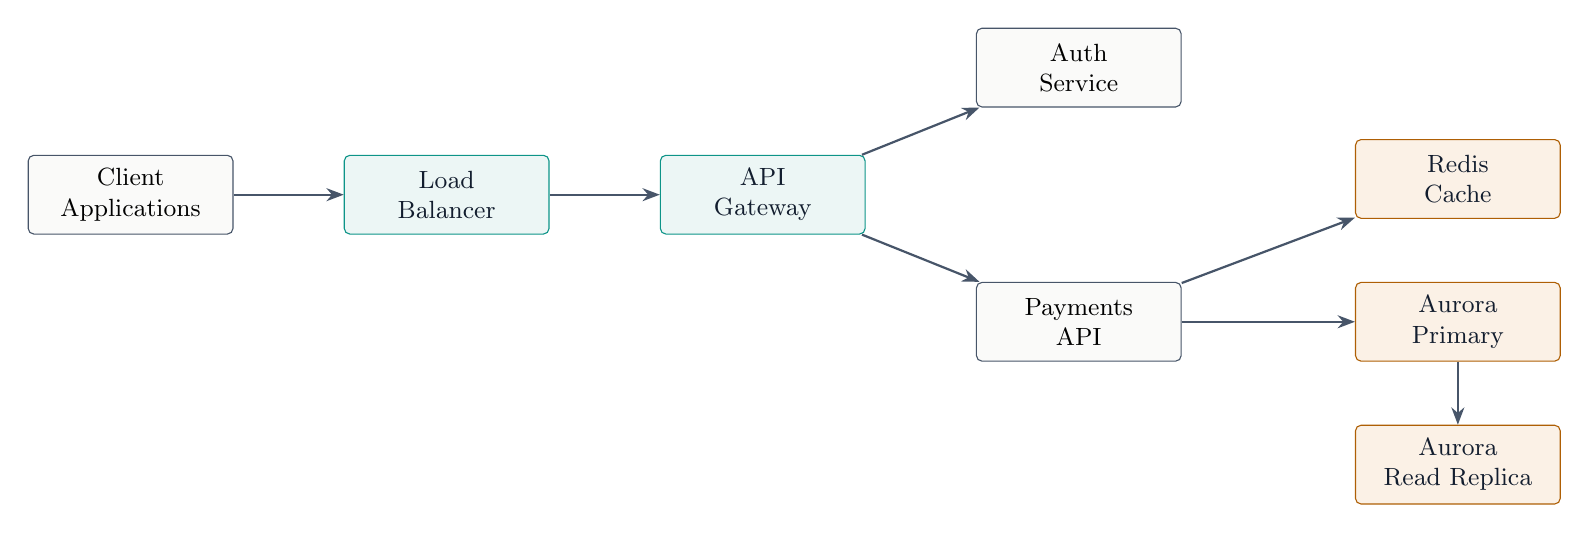
\begin{tikzpicture}[
  node distance=9mm and 14mm,
  box/.style={rectangle, rounded corners=2pt, draw=slate, fill=paper,
    minimum width=2.6cm, minimum height=1cm, align=center, font=\small},
  accent/.style={box, draw=teal, fill=teal!8, text=navy},
  data/.style={box, draw=amber!80!black, fill=amber!10, text=navy},
  arr/.style={-{Stealth[length=2.2mm]}, draw=slate, thick}
]
  \node[box] (client) {Client\\Applications};
  \node[accent, right=of client] (lb) {Load\\Balancer};
  \node[accent, right=of lb] (gw) {API\\Gateway};
  \node[box, above right=6mm and 14mm of gw] (auth) {Auth\\Service};
  \node[box, below right=6mm and 14mm of gw] (pay) {Payments\\API};
  \node[data, right=22mm of pay] (db) {Aurora\\Primary};
  \node[data, below=8mm of db] (replica) {Aurora\\Read Replica};
  \node[data, above=8mm of db] (cache) {Redis\\Cache};

  \draw[arr] (client) -- (lb);
  \draw[arr] (lb) -- (gw);
  \draw[arr] (gw) -- (auth);
  \draw[arr] (gw) -- (pay);
  \draw[arr] (pay) -- (db);
  \draw[arr] (pay) -- (cache);
  \draw[arr] (db) -- (replica);
\end{tikzpicture}
\end{center}

\begin{tabularx}{\linewidth}{@{}l X@{}}
\toprule
\textbf{Cluster} & \texttt{nexa-prod-use1} (Kubernetes 1.29, 3 node pools) \\
\textbf{Namespace} & \texttt{payments} \\
\textbf{Deployment} & \texttt{nexa-payments-api} (min 6 / max 24 replicas, HPA on CPU + queue depth) \\
\textbf{Database} & Aurora PostgreSQL 15, cluster \texttt{nexa-pay-aurora-prod} \\
\textbf{Cache} & Redis 7, cluster \texttt{nexa-pay-cache-prod} \\
\textbf{Dashboards} & Grafana: \texttt{grafana.nexa.internal/d/payments-overview} \\
\bottomrule
\end{tabularx}

% ----------------------------- Section 2 -----------------------------
\section{Escalation \& Contacts}

\begin{tabularx}{\linewidth}{@{}l l l X@{}}
\toprule
\rowcolor{navy!85}
\textcolor{white}{\textbf{Role}} & \textcolor{white}{\textbf{Name}} & \textcolor{white}{\textbf{Contact}} & \textcolor{white}{\textbf{Response Window}} \\
\midrule
On-call Primary & Marcus Webb & PagerDuty: \texttt{payments-primary} & 5 min (SEV1/2) \\
\rowcolor{navy!4}
On-call Secondary & Priya Anand & PagerDuty: \texttt{payments-secondary} & 15 min \\
Engineering Manager & David Kim & \texttt{david.kim@nexa.io} & 30 min (SEV1 only) \\
\rowcolor{navy!4}
Incident Commander & Rotation -- see IC calendar & Slack: \texttt{\#ic-oncall} & Immediate \\
Database On-call & Sofia Reyes & PagerDuty: \texttt{db-oncall} & 15 min \\
\bottomrule
\end{tabularx}

\begin{notebox}
All SEV1 and SEV2 incidents must be declared in Slack channel \texttt{\#incidents} using
the \texttt{/incident} command \emph{before} remediation begins. This creates the incident
record, timeline, and a dedicated bridge automatically.
\end{notebox}

% ----------------------------- Section 3 -----------------------------
\section{Standard Operating Procedures}

\subsection{Deploying a New Release}

Deployments to \texttt{nexa-prod-use1} run through the canary pipeline. Do not deploy
directly with \texttt{kubectl apply} outside of a declared incident.

\begin{enumerate}[leftmargin=*]
  \item Confirm the release build passed staging soak (minimum 30 minutes, error rate under 0.1\%).
  \item Trigger the canary rollout from the deploy pipeline.
  \item Watch the canary dashboard for 10 minutes; canary receives 5\% of production traffic.
  \item Promote to full rollout only if p99 latency and error rate stay within baseline.
\end{enumerate}

\begin{cmdbox}
\# 1. Verify current rollout status\\
kubectl -n payments rollout status deployment/nexa-payments-api\\
\\
\# 2. Trigger canary (5\% traffic weight)\\
nexactl deploy start --service payments-api --version v2.114.0 --canary 5\\
\\
\# 3. Watch canary error budget in real time\\
nexactl deploy watch --service payments-api --window 10m\\
\\
\# 4. Promote to 100\% once green\\
nexactl deploy promote --service payments-api
\end{cmdbox}

\subsection{Scaling the Service}

The horizontal pod autoscaler handles routine load. Manual scaling is only for
anticipated traffic spikes (e.g. merchant promotions) or HPA misbehavior.

\begin{cmdbox}
\# Inspect current HPA state\\
kubectl -n payments get hpa nexa-payments-api\\
\\
\# Temporarily raise the floor ahead of a known traffic event\\
kubectl -n payments patch hpa nexa-payments-api \textbackslash\\
\ \ -p '\{"spec":\{"minReplicas":14\}\}'\\
\\
\# Revert once the event has passed\\
kubectl -n payments patch hpa nexa-payments-api \textbackslash\\
\ \ -p '\{"spec":\{"minReplicas":6\}\}'
\end{cmdbox}

\subsection{Rotating Database Credentials}

\begin{warnbox}
Credential rotation triggers a rolling pod restart. Perform only during the
posted maintenance window (Tuesdays 02:00--03:00 UTC) unless responding to a
suspected credential leak.
\end{warnbox}

\begin{cmdbox}
\# 1. Issue new credentials in Vault\\
vault write database/rotate-root/nexa-pay-aurora-prod\\
\\
\# 2. Sync the Kubernetes secret from Vault\\
nexactl secrets sync --cluster nexa-prod-use1 --secret pay-db-creds\\
\\
\# 3. Roll the deployment to pick up the new secret\\
kubectl -n payments rollout restart deployment/nexa-payments-api
\end{cmdbox}

% ----------------------------- Section 4 -----------------------------
\section{Incident Response}

\subsection{Severity Classification}

\begin{tabularx}{\linewidth}{@{}l l X l@{}}
\toprule
\rowcolor{navy!85}
\textcolor{white}{\textbf{Level}} & \textcolor{white}{\textbf{Impact}} & \textcolor{white}{\textbf{Example}} & \textcolor{white}{\textbf{Ack SLA}} \\
\midrule
\sevbadge{crimson}{SEV1} & Full outage or data loss risk & Payments API returning 5xx cluster-wide & 5 min \\
\rowcolor{navy!4}
\sevbadge{amber}{SEV2} & Major degradation & p99 latency above 3s, partial region failure & 15 min \\
\sevbadge{teal}{SEV3} & Minor, contained impact & Single pod crash-looping, one merchant affected & 1 hour \\
\rowcolor{navy!4}
\sevbadge{slate}{SEV4} & No customer impact & Non-critical alert, capacity warning & Next business day \\
\bottomrule
\end{tabularx}

\subsection{General Incident Workflow}

\begin{enumerate}[leftmargin=*]
  \item \textbf{Acknowledge} the page in PagerDuty within the SLA for the assessed severity.
  \item \textbf{Declare} the incident via \texttt{/incident} in Slack; this opens \texttt{\#inc-\{id\}} and a Zoom bridge.
  \item \textbf{Assess} severity using the table above; adjust as new information arrives.
  \item \textbf{Mitigate} first, diagnose root cause second -- restore service, don't debug in production under fire.
  \item \textbf{Communicate} status every 15 minutes for SEV1, every 30 for SEV2, in the incident channel.
  \item \textbf{Resolve} and downgrade PagerDuty once metrics are stable for 15 consecutive minutes.
  \item \textbf{Postmortem} within 3 business days for SEV1/SEV2, posted to the incident wiki.
\end{enumerate}

\subsection{Runbook: API Latency Degradation}

\textbf{Trigger:} Alert \texttt{payments-api-p99-latency-high} fires when p99 exceeds 1.5s
for 5 consecutive minutes.

\begin{enumerate}[leftmargin=*]
  \item Check whether the Aurora primary is under connection pressure.
  \item Check whether the Redis cache hit ratio has dropped.
  \item If a recent deploy correlates with the onset, roll back immediately (Section 4.4).
\end{enumerate}

\begin{cmdbox}
\# Database connection saturation\\
nexactl db connections --cluster nexa-pay-aurora-prod\\
\\
\# Cache hit ratio over the last 30 minutes\\
nexactl cache stats --cluster nexa-pay-cache-prod --window 30m\\
\\
\# Correlate with recent deploys\\
nexactl deploy history --service payments-api --limit 5
\end{cmdbox}

\begin{dangerbox}
If Aurora primary CPU exceeds 90\% for more than 5 minutes, do \emph{not} restart the
writer instance. Failing over under load can extend the outage. Page the Database
on-call (Section 2) and force a read-replica promotion only if directed by the
Incident Commander.
\end{dangerbox}

\subsection{Rollback Procedure}

\begin{cmdbox}
\# 1. Identify the last known-good version\\
nexactl deploy history --service payments-api --limit 5\\
\\
\# 2. Roll back immediately, bypassing canary\\
nexactl deploy rollback --service payments-api --to v2.113.2 --skip-canary\\
\\
\# 3. Confirm all pods are on the rolled-back image\\
kubectl -n payments get pods -l app=payments-api \textbackslash\\
\ \ -o jsonpath='\{.items[*].spec.containers[0].image\}'\\
\\
\# 4. Watch error rate return to baseline\\
nexactl deploy watch --service payments-api --window 10m
\end{cmdbox}

% ----------------------------- Section 5 -----------------------------
\section{Monitoring \& Alert Thresholds}

\begin{tabularx}{\linewidth}{@{}X l l l@{}}
\toprule
\rowcolor{navy!85}
\textcolor{white}{\textbf{Metric}} & \textcolor{white}{\textbf{Warning}} & \textcolor{white}{\textbf{Critical}} & \textcolor{white}{\textbf{Source}} \\
\midrule
p99 latency & $>$ 800ms & $>$ 1.5s & Grafana \\
\rowcolor{navy!4}
5xx error rate & $>$ 0.5\% & $>$ 2\% & Grafana \\
Aurora CPU utilization & $>$ 75\% & $>$ 90\% & CloudWatch \\
\rowcolor{navy!4}
Redis cache hit ratio & $<$ 92\% & $<$ 80\% & Grafana \\
Pod restart count (5 min) & $\geq$ 3 & $\geq$ 8 & Kubernetes \\
\bottomrule
\end{tabularx}

% ----------------------------- Appendix -----------------------------
\section{Appendix: Quick Reference}

\begin{tabularx}{\linewidth}{@{}l X@{}}
\toprule
\textbf{Task} & \textbf{Command} \\
\midrule
Tail live logs & \texttt{nexactl logs tail --service payments-api} \\
Open a shell in a pod & \texttt{kubectl -n payments exec -it \{pod\} -- /bin/sh} \\
Force a config reload & \texttt{nexactl config reload --service payments-api} \\
Check current on-call & \texttt{nexactl oncall --team payments} \\
Drain a single node & \texttt{kubectl drain \{node\} --ignore-daemonsets} \\
\bottomrule
\end{tabularx}

\vspace{6mm}
{\footnotesize\color{slate}
This runbook is reviewed quarterly by the Payments SRE team. Report inaccuracies
in \texttt{\#sre-runbooks} or open a pull request against the \texttt{runbooks} repository.
}

\end{document}
